\documentclass[11pt]{article}

\usepackage{graphicx, amsmath, amsfonts, amssymb, microtype, fullpage, url, algorithm, algorithmic, hyperref, longtable}
\newcommand{\argmax}{\operatornamewithlimits{argmax}} 
\setlength{\parskip}{5pt}

\title{Project Report - Classification of questions on stackoverflow\\ Machine Learning, Fall 2012}
\author{Luke Vilnis, Annamalai Natarajan, Ariel Kobren}

\begin{document}
\sloppy

\maketitle
\tableofcontents
\pagebreak

\section{Problem Statement}
\begin{itemize}
\item What is a closed question?
\item Why would a question be closed?
	\begin{itemize}
	\item Exact duplicate - dropping closed questions in this category
	\item Off-topic
	\item Not constructive
	\item Note a real question
	\item Too localized
	\end{itemize}
\item What are the challenges in this problem?
	\begin{itemize}
	\item Finding closed questions
	\item Sizeable chunk of closed question is code (which is stripped off)
	\item Class label imbalance
	\end{itemize}
\end{itemize}

\section{Data set}
\begin{itemize}
\item Used data explorer on stack overflow to get the data
\item SuperCSV
\item We have 100k Questions; 50k closed, 50k open
\end{itemize}

\subsection{Pre-processing}
\begin{itemize}
\item Remove <code>
\item Remove HTML
\item Remove “cheating” features that proxy the ground truth (like “exact duplicate”)
\end{itemize}

\subsection{Features}
\begin{itemize}
\item How did we extract features from questions?
\item bucketed question length
\item presence of html tags (blockquote, code, url, etc)
\item question tags and cross products of those tags with word features
\item Stanford tokenizer 
\item Ngrams didn’t help - need smarter features - we get 100\% almost train set accuracy, so the problem is bad features, not inability to fit. Regularization also doesn’t help much at all (tried manually grid searching l2 lambda). Overfitting is not the problem.
\end{itemize}

\section{Methods}
\begin{itemize}
\item using factorie facilities for storing instances, trimming domains, learning classifiers, judging accuracy, info gain, etc. Need sparse vectors cause lots of data. pretty fast sgd implementations
\item Use information gain to see suspicious features
\end{itemize}

\section{Results}
\begin{itemize}
\item 71\% accuracy with logistic regression trained using AdaGrad (not l2 regularized but effectively regularized since its an online learning algorithm). SVM, naive bayes, l2 log reg etc does slightly worse. 
\item Naive bayes was winner until we added cross product features. High bias/low variance does better
\end{itemize}

\begin{figure}
\centering
\fbox{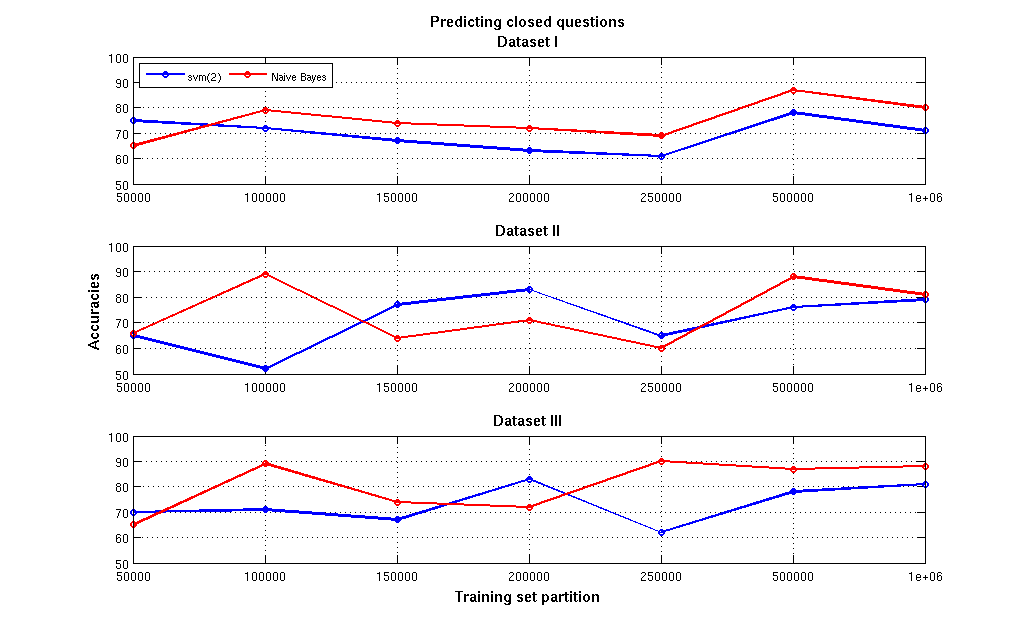
\includegraphics[width=6.5in,height=6in]{stackoverflow_results}}
\caption{Classifier accuracies in predicting closed questions}
\label{fig:results}
\end{figure}

\section{Future directions}
\begin{itemize}
\item Use kaggle data set (which we have); 70 million training instances, 80 thousand test instances
\item We’ll need to split up the data (because it’s big) to be able to use it; we’re planning to learn the weights of our linear classifier using stochastic gradient descent (blocked-adagrad)
\item Add more features (TFIDF, other NLP features), heuristic of adding number of rare words from Alex’s paper
\item Try out new classifiers - random forests
\item Try things besides open/closed - like answered/unanswered
\end{itemize}

\end{document}

